\subsection{Theorie des Quantentunnelns}
\textit{Quantentunneln}, oder kurz \textit{Tunneln} 
bezeichnet das quantenmechanische Phänomen, wenn 
die Durchtrittswahrscheinlichkeit eines Teilchens
durch eine Potenzialbarriere nicht null ist, selbst wenn die Energie
des Teilchens geringer ist als das Potenzial selbst ($E < V$), was
in der klassischen Mechanik nicht möglich wäre. Dies
spielt eine wichtige Rolle bei
vielen Phänomenen in Natur und Technik,
beispielsweise bei der Kernfusion der Sonne, bei der Diode und
daher auch beim Transistor und somit bei der Funktionionsweise
eines Computers an sich, aber auch beim Quantencomputer oder
eben in unserem Fall beim RTM. Das Phänomen des Quantentunnelns
wurde Anfang des 20ten Jahrhunderts mit der Entdeckung der 
Quantenmechanik postuliert und Mitte des Jahrhunderts bestätigt.
\subsection{Mathematische Herleitung von Quantentunneln}
In den folgenden Ausführungen werden Kenntnisse der Quantenmechanik
vorrausgesetzt. Betrachten wir zunächst die Zeitunabhängige
Schrödingergleichung für ein Teilchen in einer Dimension:
\begin{align}
\left [ \frac{-\hbar^2}{2m}\partial_x^2 + V(x) \right ]\psi(x) = E\psi(x) \\ 
\Leftrightarrow \left [ \frac{-\hbar^2}{2m}\partial_x^2 \right ]\psi(x) = \left [E-V(x) \right ]\psi(x) 
\end{align}
Im Spezialfall wenn $V(x)$ konstant ist, können wir die Gleichung
sofort mit planaren Wellen lösen:
\begin{align}
    k^2 = \frac{2m}{\hbar^2}(V-E)\\
    \psi(x) \sim \exp(ikx) 
\end{align}
\subsubsection{Rechteckspotenzial}
Nehmen wir nun an, das Potenzial ist gegeben durch:
\begin{equation}
    V(x) = V_0 \left [ \Theta(x) - \Theta(x-a) \right ] 
\end{equation}
Wobei $\Theta(x)$ die Heavisidefunktion ist und $V_0 > E$.
Die Barriere teilt den Raum nun in drei Teile, $x<0$, $0\leqslant x\leqslant a$ und $a<x$.
In jedem dieser Teile ist das Potenzial konstant, somit können wir für jeden Teil eine
obere Lösung ansetzen \cite{wolfgang2010experimentalphysik},
\cite{landau1991quantenmechanik}:
\begin{align}
    \psi_I(x)    &= A_r \exp(ik_0x) + A_l  \exp(-ik_0x) \mbox{ for } x<0\\
    \psi_{II}(x) &= B_r \exp(ik_1x) + B_l  \exp(-ik_1x) \mbox{ for } 0 \leqslant x \leqslant a\\
    \psi_{III}(x)&= C_r \exp(ik_0x) + C_l  \exp(-ik_0x) \mbox{ for } x>0
\end{align}
Für $E>V_0$ gilt nun:
\begin{align}
    k_0 &= \frac{\sqrt{2mE}}{\hbar}\\
    k_1 &= \frac{\sqrt{2m(E-V_0)}}{\hbar}
\end{align}
Die Koeffizienten A,B und C lassen sich nun mit den Randbedingungen
für die Stetigkeit lösen:
\begin{align}
    \psi_I(0)&\overset{!}{=} \psi_{II}(0)\\
    (\partial_x\psi_I)(0)&\overset{!}{=} (\partial_x\psi_{II})(0)\\
    \psi_{II}(a)&\overset{!}{=} \psi_{III}(a)\\
    (\partial_x\psi_{II})(a)&\overset{!}{=} (\partial_x\psi_{III})(a)
\end{align}
Dies ergibt nach einsetzen der Lösungen für die Wellenfunktionen:
\begin{align}
  A_r + A_l &= B_r + B_l \\
  ik_0(A_r-A_l) &= ik_1(B_r-B_l)\\
  B_r\exp(iak_1)+B_l\exp(-iak_1)&=C_r \exp(iak_0)+C_l\exp(-iak_0)\\
  ik_1(B_r\exp(iak_1) - B_l\exp(-iak_1))&=ik_0(C_r\exp(iak_0)-C_l\exp(-iak_0))
\end{align}
Dies sind 6 freie Parameter für 4 Gleichungen, also können wir zwei 
Paramter festsetzen. Wir setzen $A_r =1$ (Skalierung nach der einlaufenden
Welle) und $C_l = 0$, das bedeutet, dass keine Welle von rechts dazukommt,
sondern alles von der einlaufenden Welle $A_r$ abhängt. Des weiteren
benennen wir $A_l=r$ für Reflexion, und $C_r=t$ für Transmission. Nun
lassen sich die Gleichungen nach diesen Koeffizienten auflösen:
\begin{align}
    t &= \frac{4k_0k_1\exp(-ia(k_0-k_1))}{(k_0+k_1)^2 - \exp(2iak_1)(k_0-k_1)^2}\\
    r &= \frac{(k_0^2 - k_1^2)\sin(ak_1)}{2ik_0k_1\cos(ak_1)+(k_0^2+k_1^2)\sin(ak_1)}
\end{align}
Nun lässt sich mit diesen Ausdrücken die Übergangswahrscheinlichkeit durch die 
Barriere berechnen:
\begin{align}
    T = \left | t \right |^2 = \frac{1}{1 + \frac{V_0^2 \sinh^2(k_1a)}{4E(V_0-E)}}
    \label{eq:T1}
\end{align}
Wenn das Potenzial kleiner ist als die Energie, läuft die Rechung analog
(wobei $k_1 = \frac{\sqrt{2m(V_0-E)}}{\hbar}$) und wir erhalten:
\begin{align}
    T = \left | t \right |^2 = \frac{1}{1 - \frac{V_0^2 \sin^2(k_1a)}{4E(V_0-E)}}
    \label{eq:T2}
\end{align}

\begin{figure}
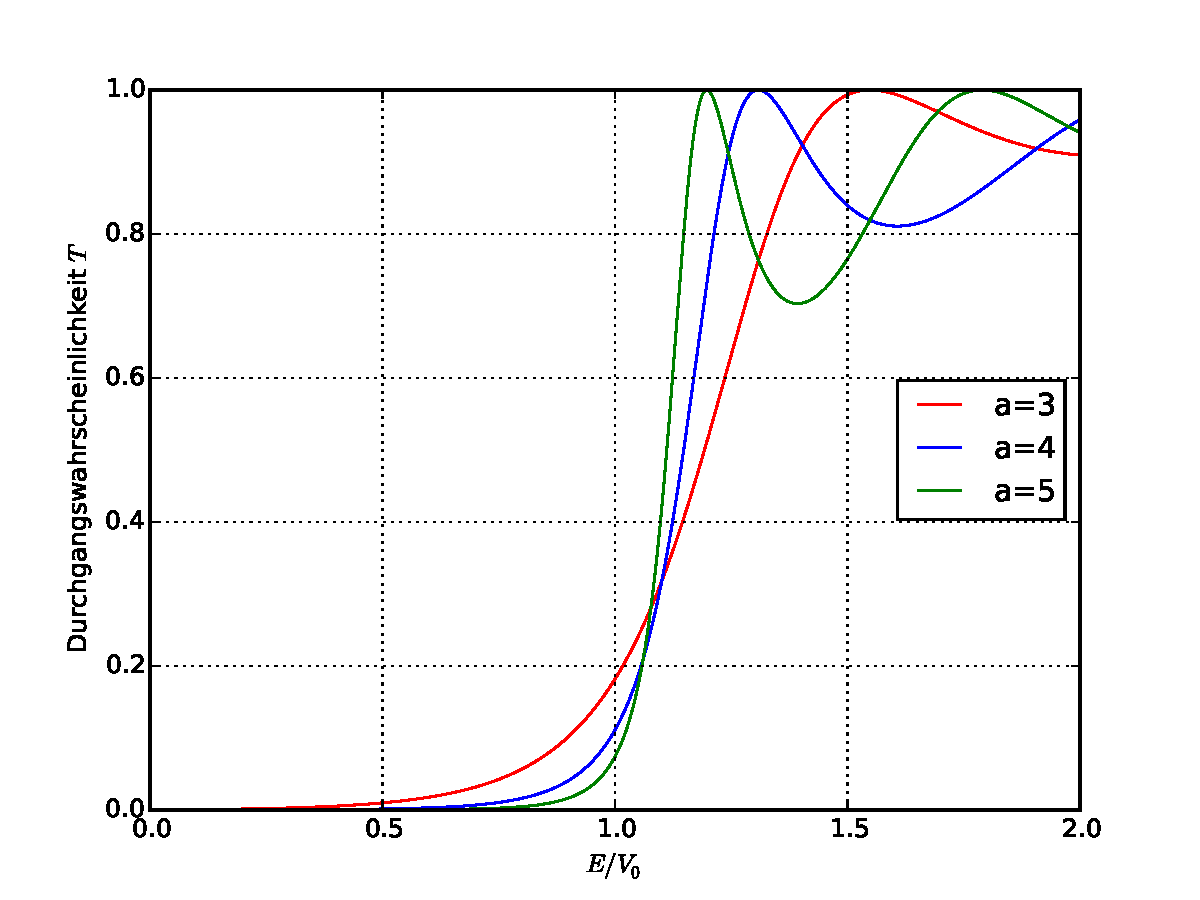
\includegraphics[width=14cm]{pics/tunnel1}
\caption{Transmissionswahrscheinlichkeit nach Gleichung~\ref{eq:T1} und Gleichung~\ref{eq:T2}
bei verschiedenen Breiten des Potenzials $a$ (obdA wurde hier $\hbar=1$ und $m=1$ gewählt).
Hier wird deutlich ersichtlich, inwiefern sich der Quantenmechanische Fall vom klassischen
Fall unterscheidet, so ist die Wahrscheinlichkeit für Energien kleiner als das Potenzial ungleich
null und auch bei höheren Energien nicht konstant eins.} 
 \label{fig:tunnel1}
\end{figure}

\subsubsection{Tunneleffekt beim Rastertunnelmikroskop}
Im eben besprochenen Fall der eindimensionalen Potenzialwand zeichnet sich schon das
assymptotische Verhalten für $a\gg1$ ab:
\begin{equation}
    T = \left | t \right |^2 \overset{\kappa a \gg 1}{\rightarrow} (\frac{4k_1k_0}{k_1^2+k_0^2})^2 
    \exp(-2k_1a)
\end{equation}
Dies ist unter den vielen Bedingungen nur eine grobe Näherung für die Tunnelmikroskopie, doch
wir werden später sehen, dass diese Näherung gut mit einem detaillierteren Ansatz übereinstimmt.
